\documentclass{ximera}  
\title{If/Else Statements}  
\begin{document}  
\begin{abstract}  
We introduce if/else statements in Python.
\end{abstract}  
\maketitle

\section{If/Else}

In an earlier section we saw that in order to compute the absolute value of a real number $x$, we first needed to determine if it satisfied a certain condition, namely, is it the case that $x>0$? The answer to this question then determines the set of instructions to follow. We can reformulate our algorithm for computing $|x|$ as two statements in the following way:

For any real number $x$, if $x>0$, then $|x|=x$. Else (or otherwise), $|x|=-x$.

The `if' portion of the statement explains what to do if the given condition is satisfied, while the `else' portion explains what to do if the given condition is not satisfied. This can be easily mapped to the flowchart for computing $|x|$ below.

\begin{center}
	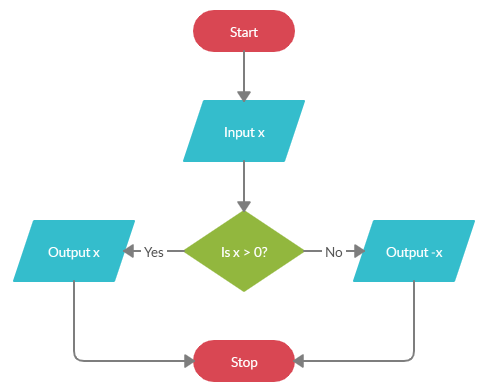
\includegraphics{absalgo.png}
\end{center}

In Python we can implement this short algorithm using the following syntax:

\noindent\rule{\textwidth}{1pt}
\begin{verbatim}
if condition:
        code1
else:
        code2
\end{verbatim}
\noindent\rule{\textwidth}{1pt}

The term \verb|condition| indicates the condition we wish to check. If the condition evaluates to \verb|True|, then the instructions given by \verb|code1| are followed. If the condition evaluates to \verb|False|, then the instructions given by \verb|code2| are followed. Using the template above, we can now write the necessary Python code to compute $|x|$.
      
\noindent\rule{\textwidth}{1pt}    
\begin{verbatim}
if x > 0:
        absVal = x
else:
        absVal = -x
\end{verbatim}
\noindent\rule{\textwidth}{1pt}

The code above creates a variable \verb|absVal| that is assigned the absolute value of $x$ for any given $x$. The SageCell below shows how to use this code in practice.

\begin{sageCell}
x = -3               # change this value and evaluate the cell to compute |x| for other x values

if x > 0:
	absVal = x
else:
	absVal = -x
print(absVal)        # this line prints the value of abs to the screen to show that the variable has been assigned the correct value
\end{sageCell}

Note that in Python, whitespace (indentation) determines which lines of code belong to a particular code block. For example, the following code differs from that in the SageCell above in that the \verb|print| statement is only called if $x\leq 0$.

\begin{sageCell}
x = 4

if x > 0:
	absVal = x
else:
	absVal = -x
	print(absVal)
\end{sageCell}

The example above shows how a flowchart with a decision compartment can be translated to Python code and vice versa. With enough practice one shoud be able to go between the two. Eventually, with enough experience, one can start coding without explicitly drawing a flowchart each time.

\section{Elif}

Below we give examples of how to expand on the basic if/else form to handle cases where multiple decisions are needed or if a decision has more than two outcomes. 

Let $sgn$ be the sign function. For any real number $x$, $sgn(x)$ is $+1$ if $x>0$, -1 if $x<0$, and $0$ otherwise. The flowchart below shows a possible algorithm for computing this function.

\begin{center}
	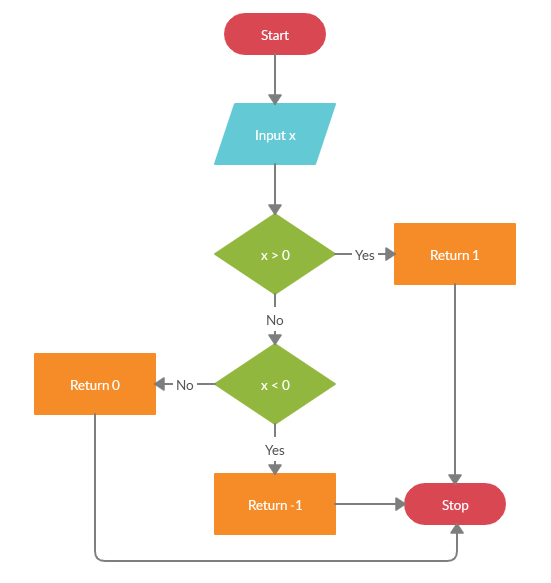
\includegraphics{signfun.png}
\end{center}

This can be implemented in Python in several ways. 

We can put an if/else statement inside of another if or else block of code. Note the indentation of the lines belonging to the second if/else statement.

\begin{sageCell}
x = -5
if x > 0:
	sgn = 1
else:
	if x < 0:
		sgn = -1
	else:
		sgn = 0
print(sgn)
\end{sageCell}
	
We can use the \verb|elif| (else-if) option that simply shortens the code above.

\noindent\rule{\textwidth}{1pt}
\begin{verbatim}
if condition1:
        code1
elif condition2:
        code2
elif condition3:
        code3
    ...
elif conditionk:
        codek
else:
        code(k+1)
\end{verbatim}
\noindent\rule{\textwidth}{1pt}

The \verb|elif| lines above allow one to write a program that checks multiple conditions. The program will execute whatever instructions are associated with the first (and only the first) condition checked that is satisfied. If none of the conditions are satisfied, then the default behavior is given by the code in the \verb|else| portion.

\begin{sageCell}
x = 4
if x > 0:
        sgn = 1
elif x < 0:
        sgn = -1
else:
        sgn = 0
print(sgn)
\end{sageCell}

Note that the second option greatly increases the readability of the code and can be expanded with more \verb|elif| lines if more options must be considered.

\section{Problems}

\begin{question}
Define the Heavyside step function $H$ for any real number $x$ as
	$$H(x)=\begin{cases} 1 &\text{ if $x\geq 0$}\\
		0 &\text{ otherwise.}
	\end{cases}$$
Create an algorithm to implement the Heavyside function. Express your algorithm as a flowchart and in Python.
	\begin{hint}
		This problem is similar to computing $|x|$. Note that the second hint for this problem is the solution.
	\end{hint}
	\begin{hint}
	\begin{center}
		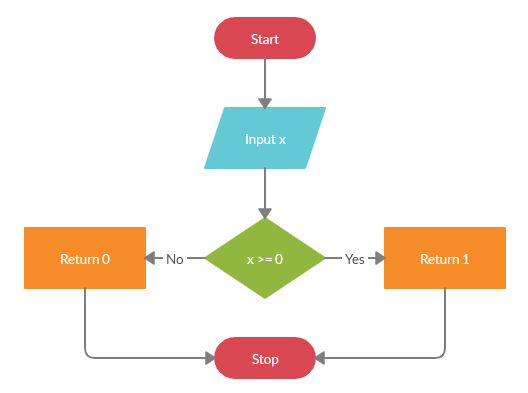
\includegraphics{heavy.png}
	\end{center}
\begin{sageCell}
if x >= 0:
        H = 1
else:
        H = 0
\end{sageCell}
	\end{hint}
\end{question}

\begin{question}
A different definition of the Heavyside step function gives a different value at $x=0$, namely,
	$$H(x)=\begin{cases} 1 &\text{ if $x>0$}\\
		1/2 &\text{ if $x=0$}\\
		0 &\text{ otherwise.}
	\end{cases}$$
Create an algorithm to implement this alternative Heavyside function. Express your algorithm as a flowchart and in Python.
	\begin{hint}
		This problem is similar to computing $sgn(x)$. Note that the second hint for this problem is the solution.
	\end{hint}
	\begin{hint}
	\begin{center}
		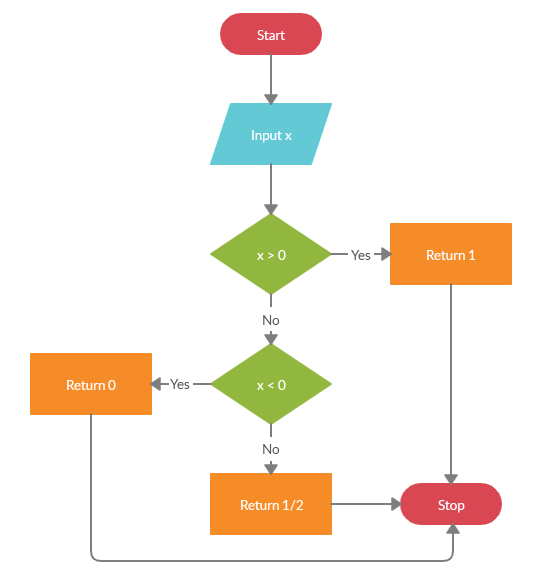
\includegraphics{heavy2.png}
	\end{center}
\begin{sageCell}
if x > 0:
        H = 1
elif x == 0:
        H = 0.5
else:
        H = 0
\end{sageCell}
	\end{hint}
\end{question}

\end{document}
